
\documentclass{beamer}

\mode<presentation> 
	{
	%\usetheme{Berlin}
	%\usetheme{Copenhagen}
	%\usetheme{Luebeck}
	\usetheme{Madrid}
	\setbeamertemplate{navigation symbols}{} 
	\setbeamertemplate{itemize item}[square]
	\setbeamertemplate{itemize subitem}[square]
	\setbeamerfont{footnote}{size=\tiny}
	}

\usepackage{graphicx} 
\usepackage{booktabs} 
\usepackage{amsmath,amssymb}

%----------------------------------------------------------------------------------------
%	TITLE PAGE
%----------------------------------------------------------------------------------------

\title[Activity Patterns in Network Communities]{Activity Patterns in Social Network Communities:  \\ a study on scale invariance} 

\author{Matteo Garbellini} 
\institute[Unimi] 
{
Universit\`a degli Studi di Milano \\ 
\medskip
\textit{matteo.garbellini@studenti.unimi.it} 
}
\date{23 Luglio 2019} 

\begin{document}

\begin{frame}
\titlepage 
\end{frame}

\begin{frame}
\frametitle{Overview} % Table of contents slide, comment this block out to remove it
\tableofcontents % Throughout your presentation, if you choose to use \section{} and \subsection{} commands, these will automatically be printed on this slide as an overview of your presentation
\end{frame}

%----------------------------------------------------------------------------------------
%	PRESENTATION SLIDES
%----------------------------------------------------------------------------------------

%------------------------------------------------
\section{Introduction} 

\subsection{question}
\subsection{dataset} 

\section{Theoretical Aspects}
\subsection{community detection}
\subsection{resolution parameter}
\subsection{intertime and spike trains}

\section{Computational Aspects}
\subsection{tools}
\subsection{process}
\section{Results}
\subsection{normalized activity}
\subsection{intertime}
\subsection{node activity}
\section{Conclusions and Further Developments}


%------------------------------------------------
\begin{frame}
\frametitle{Introduction}
\begin{block}{Question}
Do differently sized communities have different patterns of activity, or are these patterns scale invariant
\end{block}

\begin{itemize}
	\item Dataset: Twitter Activity before/after the announcement of the discovery of the Higgs Boson
\end{itemize}
\end{frame}

%------------------------------------------------

\begin{frame}
\frametitle{Dataset}
Twitter activity before/during/after the announcement of the discovery of the Higgs Boson on July 12th 2012


\begin{itemize}
	\item \textit{higgs-social-network.edges}: directed graph of following/followers twitter users
	\begin{itemize}
		\item 450000 nodes (users)
		\item 14 million edges (friendships)
	\end{itemize}
	\item \textit{higgs-activity-time}: timestamped interactions between users, based on type of interaction Retweet(RT), Mention (MT), and Replies (RE) 
	\begin{itemize}
		\item Time frame: July 11th 0.00am to July 12th 11.59pm
		\item 500000 events (interactions)
		\item Format: $UserA$ $UserB$ $timestamp$ $interaction$
	\end{itemize}
\end{itemize}
\end{frame}

%------------------------------------------------

\begin{frame}
\frametitle{Community Detection}
Choosing the right community detection algorithm is an important step in the dataset analysis. For large networks \textbf{modularity} based algorithms perform the best. A first analysis was done using the Louvain Algorithm, while the final results were obtained using the CPM Algorithm


\begin{itemize}
	\item Louvain Modularity Algorithm\footnotemark
	\begin{itemize}
		\item fast for large graph
		\item small communities tend to be merged
	\end{itemize}
	\item Constant Potts Model\footnotemark
	\begin{itemize}
		\item efficient \textit{Louvain} alternative
		\item almost Resolution Limit Free
		\item able to discover small sub-communities
	\end{itemize}
\end{itemize}
\footnotetext[1]{Blondel, V. D., Guillaume, J., Lefebvre, E. (2008). Fast unfolding of communities in large networks, 1–12.}
\footnotetext[2]{Traag, V. A., Dooren, P. Van, Nesterov, Y. (2011). Narrow scope for resolution-limit-free community detection.}
\end{frame}

%------------------------------------------------

\begin{frame}
\frametitle{Community Detection: Constant Potts Model}
The Constant Potts Model compares the network to a constant parameter $\gamma$ instead of a null-model like the Louvain algorithm. It works by minimizing  \\
$$\mathcal{H} = - \sum_{i,j}(A_{ij}\omega_{ij}-\gamma)\delta(\sigma_{i},\sigma_{j})$$
where $\gamma$ is the so-called \textbf{resolution parameter}. Follows the inequality $$n_{c} > \sqrt{\frac{1}{\gamma}}$$ where $n_{c}$ is the cluster size lower bound.
\end{frame}

%------------------------------------------------

\begin{frame}
\frametitle{Community Detection: Choosing the Resolution Parameter}
Choosing the resolution parameter is a delicate step of community detection
\begin{itemize}
	\item resolution profile
	\item stable partitions
	\item research-oriented lower bound size 
	\item (my case) cross-reference with \textit{Surprise Partition Algorithm}\footnotemark
\end{itemize}


\footnotetext[1]{Aldecoa, R., Marín, I. (2011). Deciphering network community structure by surprise}
\end{frame}

%------------------------------------------------

\begin{frame}
\frametitle{Community Detection: size distribution CPM vs Surprise Partition}
\begin{figure}
	\includegraphics[width=0.8\linewidth]{figures/community_size_surprise_cpm}
\end{figure}
\end{frame}

%------------------------------------------------

\begin{frame}
\frametitle{Activity Classification: Activity Index and Activation Index}
Two parameters are proposed: the \textbf{activity index} and the \textbf{activation index}, defined as follows:
\begin{itemize}
	\item Activity Index $\Lambda$  \\ $$\Lambda = \frac{Events}{ActiveNodes}$$
	\item Activation Index $\Upsilon$  \\ $$\Upsilon = \frac{Activations}{ActiveNodes}$$
\end{itemize}
\end{frame}

%------------------------------------------------

\begin{frame}
\frametitle{Activity Classification: Events Intertime}

\end{frame}


%------------------------------------------------

\begin{frame}
\frametitle{Activity Classification: Spike Trains and Local Variation}
To uncover the dynamics of communications spikes (bursts), \textbf{local variation} $L_{v}$ is applied, providing a local temporal measurment usually defined to characterize non-stationary neuron spike trains \footnotemark 

$$L_{v}=\frac{3}{N-2}\sum_{i=2}^{N-1}\bigg(\frac{(\tau_{i+1}-\tau_{i}) - (\tau_{i}-\tau_{i-1})}{(\tau_{i+1}-\tau_{i}) + (\tau_{i}-\tau_{i-1})}\bigg)^2 $$

where $N$ is the number of spikes and $\Delta\tau$ is the backward and forward delay.
\footnotetext[4]{Sanli, C., Lambiotte, R. (2015). Temporal pattern of online communication spike trains in spreading a scientific rumor : how often , who interacts with whom?}

\end{frame}

%------------------------------------------------

\begin{frame}
\frametitle{Computational Aspects: tools}

\begin{itemize}
	\item Tools Used
	\begin{itemize}
		\item Community Detection: igraph w/ Python using \textbf{leidenalg} algorithm (Traag)
		\item Community Analysis: C++ , awk and bash scripts
		\item Graphs and fits: gnuplot
	\end{itemize}
\end{itemize}
\end{frame}

%------------------------------------------------

\begin{frame}
\frametitle{Computational Aspects: process}

\begin{itemize}
	\item higgs-community-detection.py: outputs detected communities
	\item higgs-preprocess-analysis.sh: performes basics parsing and file reformat
	\item higgs-analysis.cpp: builds all necessary information on the network and outputs all graph data
\end{itemize}
\end{frame}

%------------------------------------------------

\begin{frame}
\frametitle{RESULTS: Community detection}
\textbf{Insert figure here: cluster-size vs cluster-frequency}
\begin{figure}
	%\includegraphics[width=0.8\linewidth]{figures/CPM_clustersize}
\end{figure}
\end{frame}

%------------------------------------------------

\begin{frame}
\frametitle{RESULTS: bin-size Definition}
Communities sizes are classified following this general rule \\
\begin{itemize}
	\item Very Small : $< 25$ \textbf{not considered in analysis}
	\item Small: $25-100$ 
	\item Medium: $100-1000$
	\item Large: $1000-5000$
	\item Very Large: $5000-10000$
	\item Huge: $>10^{4}$
\end{itemize}

The actual analysis is done considering log-sized bin averages. Each class has 10 sub-classes (10,20..100,200..1000,2000..)
\end{frame}

%-----------------------------------------------

\begin{frame}
\frametitle{RESULTS OVERVIEW}
\begin{itemize}
	\item \textbf{Activity by cluster size}
	\begin{itemize}
		\item ingoing / outgoing / within cluster
		\item retweet / mention / reply
		\item ingoing / outgoing / within by type (rt, re, mt)
	\end{itemize}
	\item \textbf{Average node activity by cluster size}
	\item \textbf{Average node intertime by cluster size}


\end{itemize}
\end{frame}

%------------------------------------------------

\begin{frame}
\frametitle{RESULTS: Cluster Activity }
\begin{figure}
	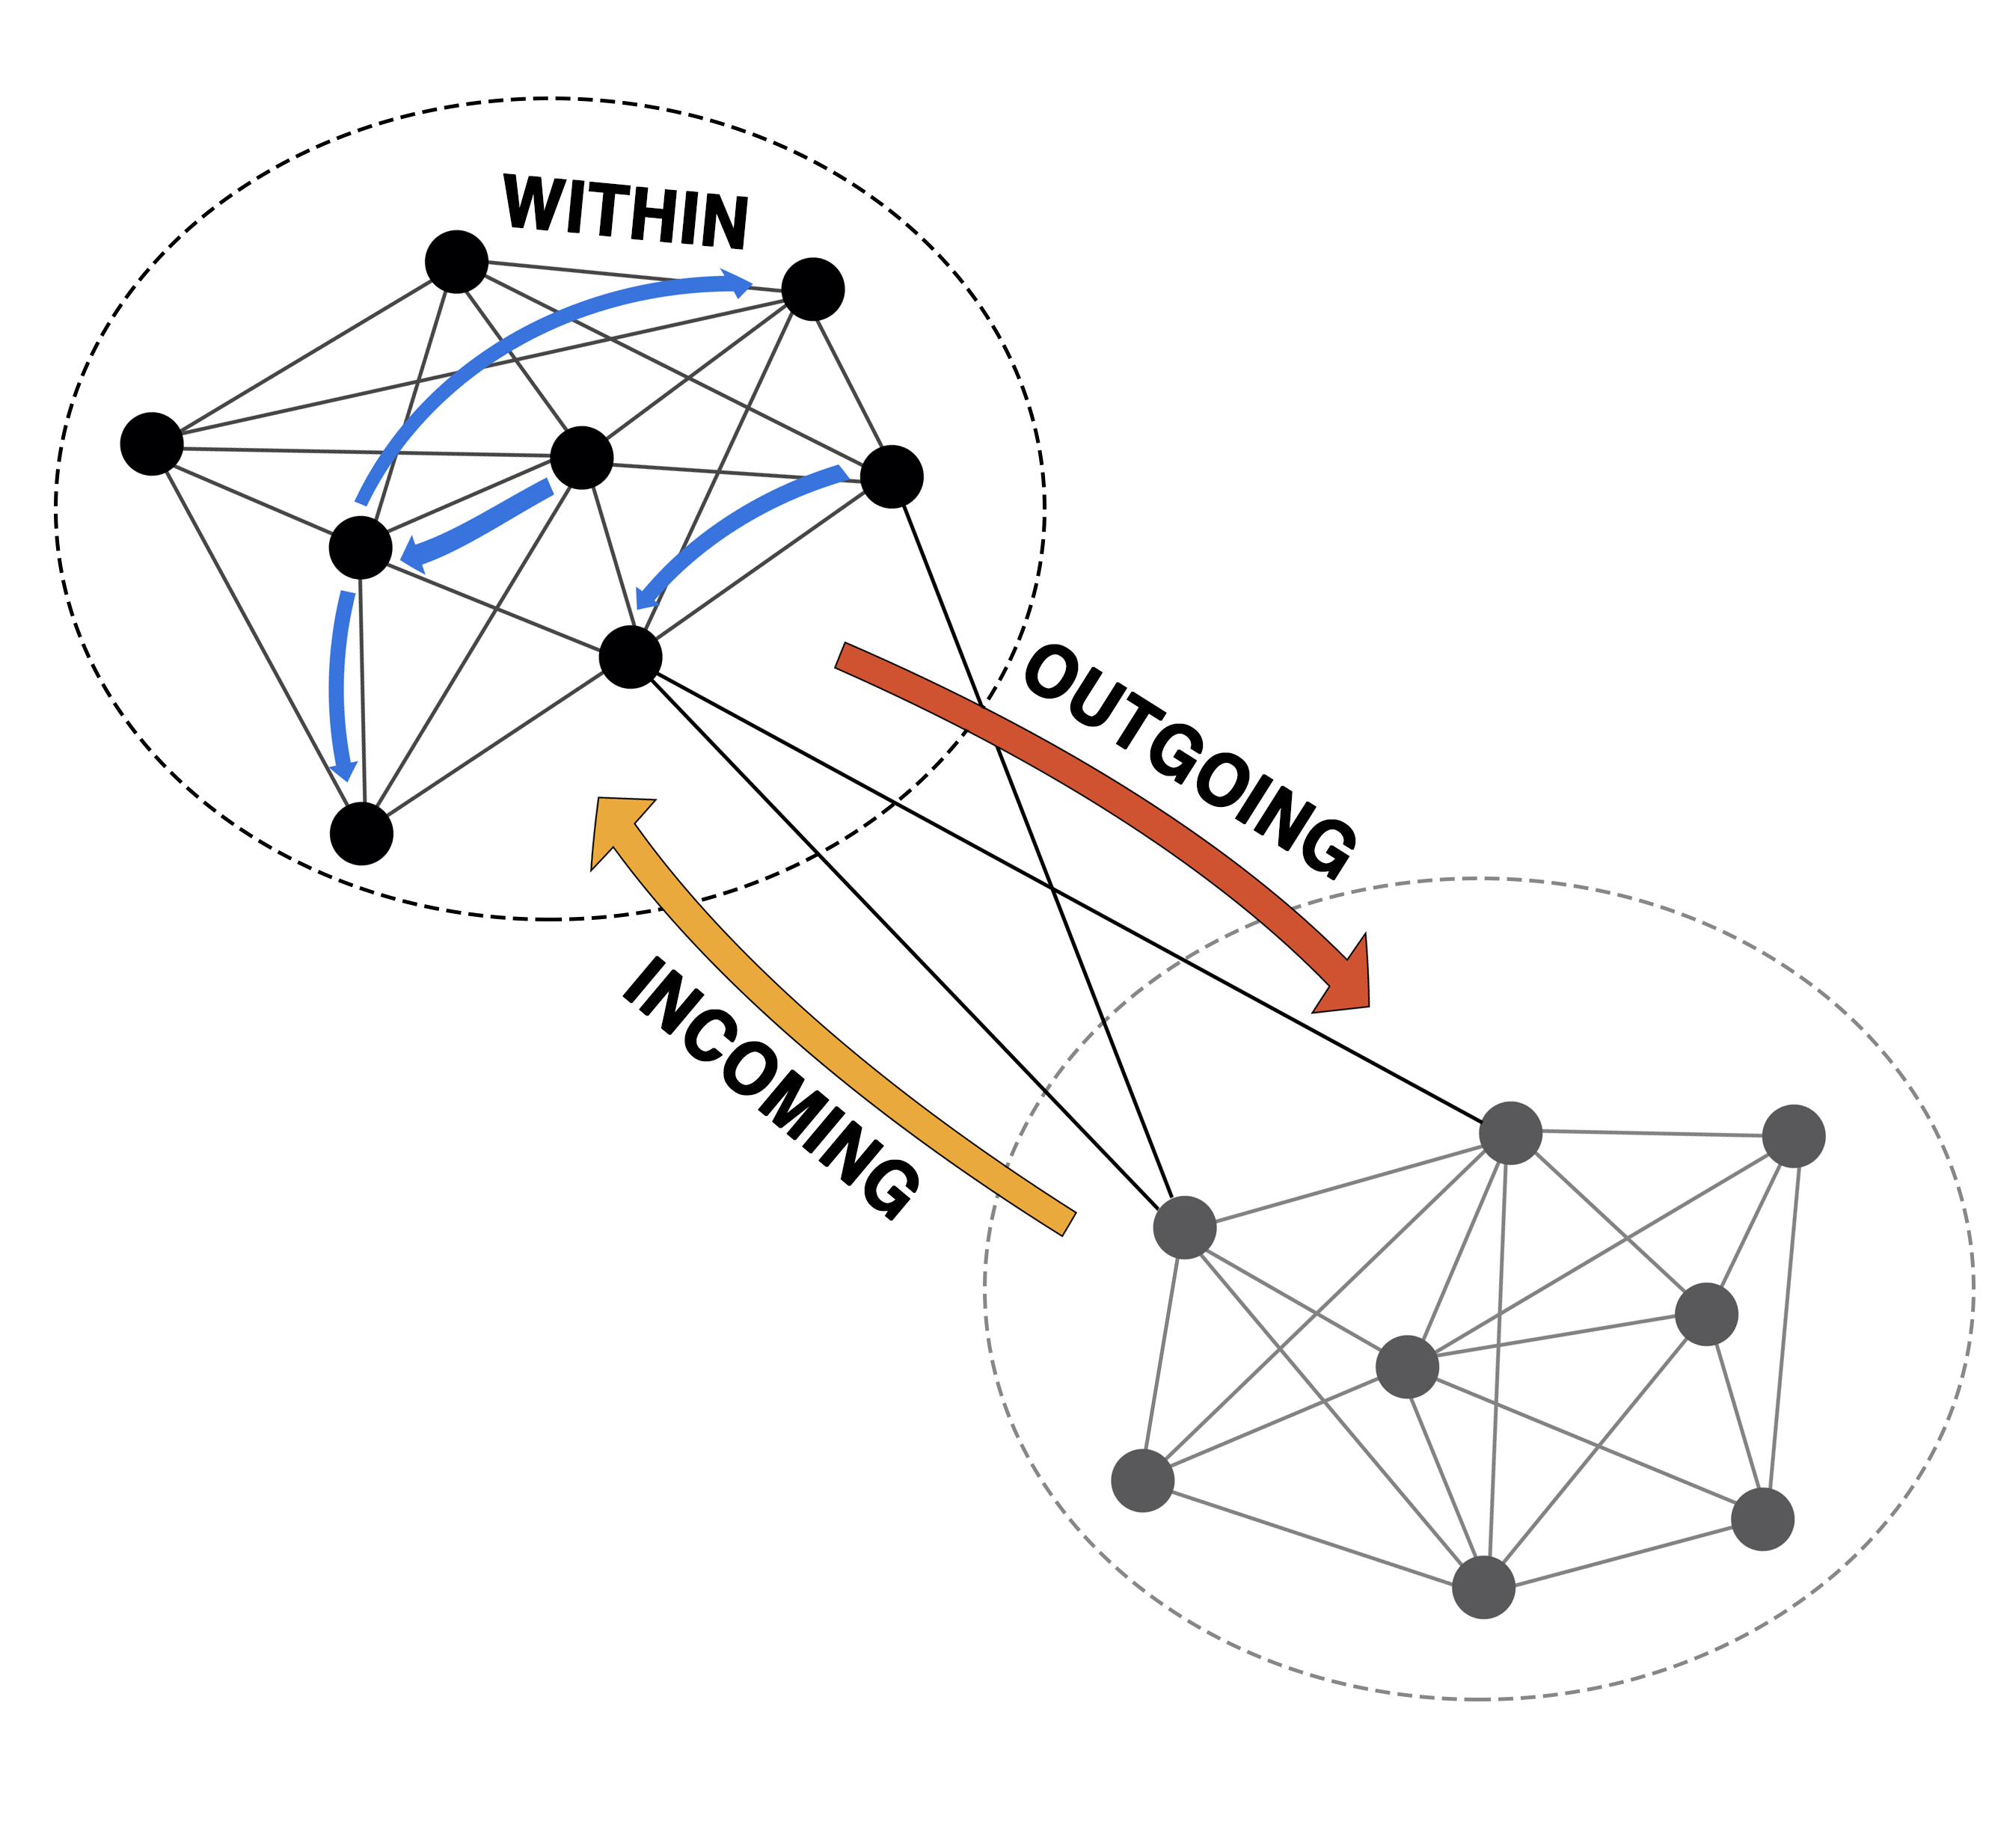
\includegraphics[width=0.8\linewidth]{figures/activity}
\end{figure}
\end{frame}


%------------------------------------------------

\begin{frame}
\frametitle{RESULTS: Cluster Activity (ingoing/outgoing/within)}
\begin{figure}
	\includegraphics[width=0.8\linewidth]{figures/activity_inout}
\end{figure}
\end{frame}

%------------------------------------------------

\begin{frame}
\frametitle{RESULTS: Cluster Activity by type}
\begin{figure}
	\includegraphics[width=0.8\linewidth]{figures/activity_bytype}
\end{figure}
\end{frame}

%-----------------------------------------------
\begin{frame}
\frametitle{RESULTS: Activity Within Cluster by type}
\begin{figure}
	\includegraphics[width=0.8\linewidth]{figures/activity_within_bytype}
\end{figure}
\end{frame}

%------------------------------------------------

\begin{frame}
\frametitle{RESULTS: Node Activation}
\begin{figure}
	\includegraphics[width=0.8\linewidth]{figures/node_activation}
\end{figure}
\end{frame}














%----------------------------------------------------------------------------------------

\end{document} 